\section{Gestión de clientes y contactos (desde cero)}

Esta parte del sistema es como tu agenda telefónica y directorio de clientes, pero mucho más potente. Aquí guardarás la información de todos los pasajeros (PAX), proveedores y agencias con las que trabajas.

% ─────────────────────────────────────────────────────────────────────────────
\subsection{Abrir la aplicación Contactos}

Para ver tu lista de contactos, primero debes entrar a la aplicación de Contactos.

\begin{figure}[H]
    \centering
    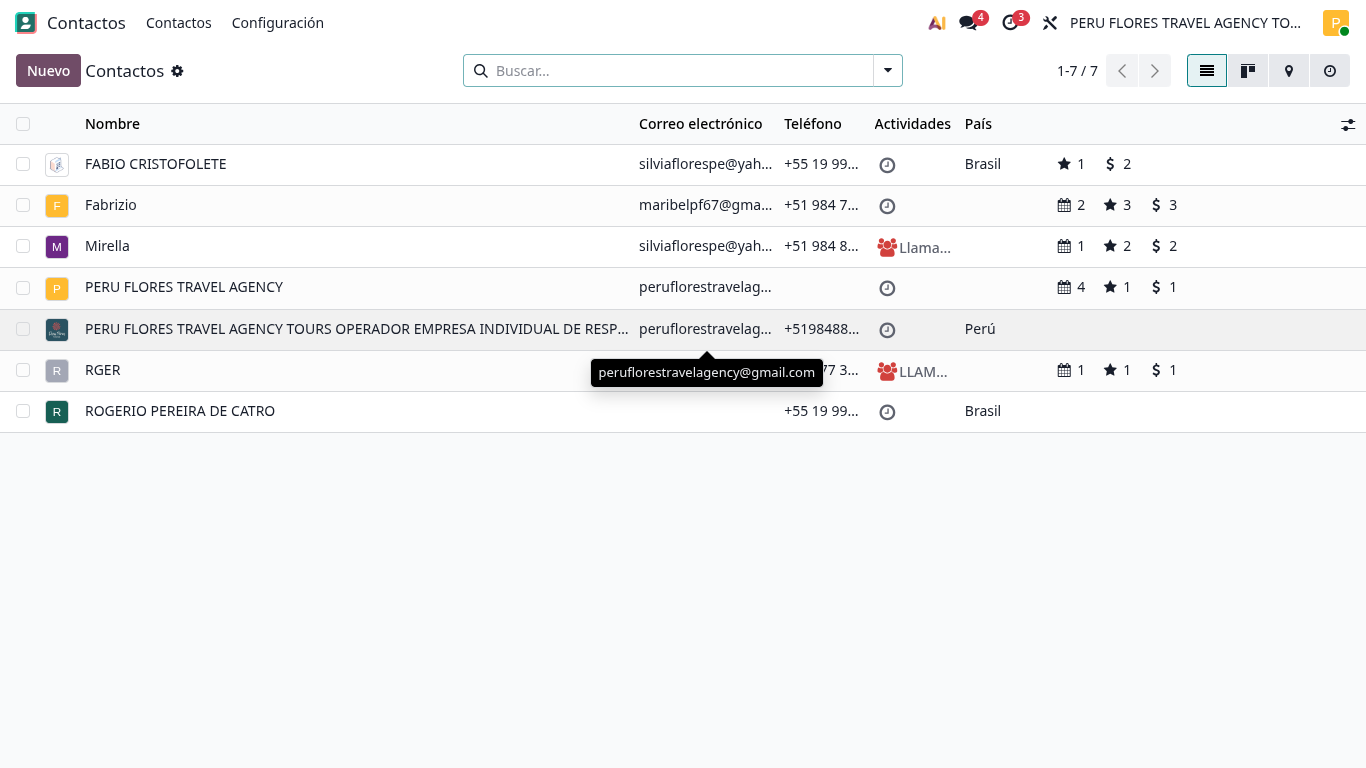
\includegraphics[width=0.9\textwidth]{assets/con_01_lista.png}
    \caption{Pantalla principal donde ves a todos tus contactos guardados}
\end{figure}

Sigue estos pasos:
\begin{enumerate}
    \item En la pantalla de inicio del sistema, busca el ícono que dice \textbf{``Contactos''} y haz clic ahí.
    \item Se abrirá una pantalla con tarjetitas o una lista, mostrando a todas las personas y empresas que ya tienes guardadas, como se ve en la imagen de arriba.
\end{enumerate}

% ─────────────────────────────────────────────────────────────────────────────
\subsection{Crear un contacto nuevo}

Si tienes un nuevo cliente o un nuevo proveedor, debes agregarlo al sistema para poder venderle o comprarle.

\begin{figure}[H]
    \centering
    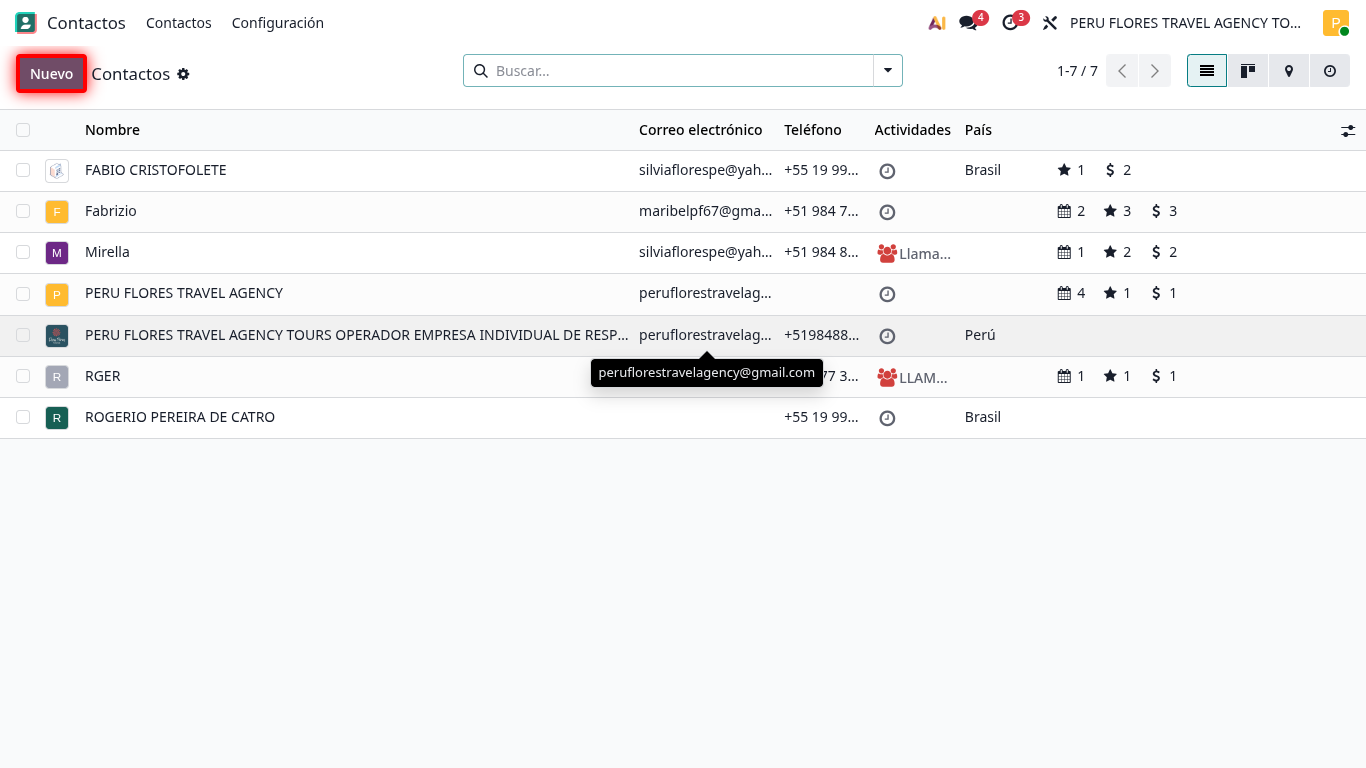
\includegraphics[width=0.9\textwidth]{assets/con_02_nuevo_highlight.png}
    \caption{El botón \textbf{``Nuevo''} (marcado en rojo) para registrar un nuevo contacto}
\end{figure}

Sigue estos pasos:
\begin{enumerate}
    \item Busca en la parte de arriba, a la izquierda, el botón que dice \textbf{``Nuevo''} (lo hemos marcado con un cuadro rojo).
    \item Haz clic ahí. Se abrirá una ficha en blanco (como la imagen de abajo) para que ingreses sus datos.
\end{enumerate}

\begin{figure}[H]
    \centering
    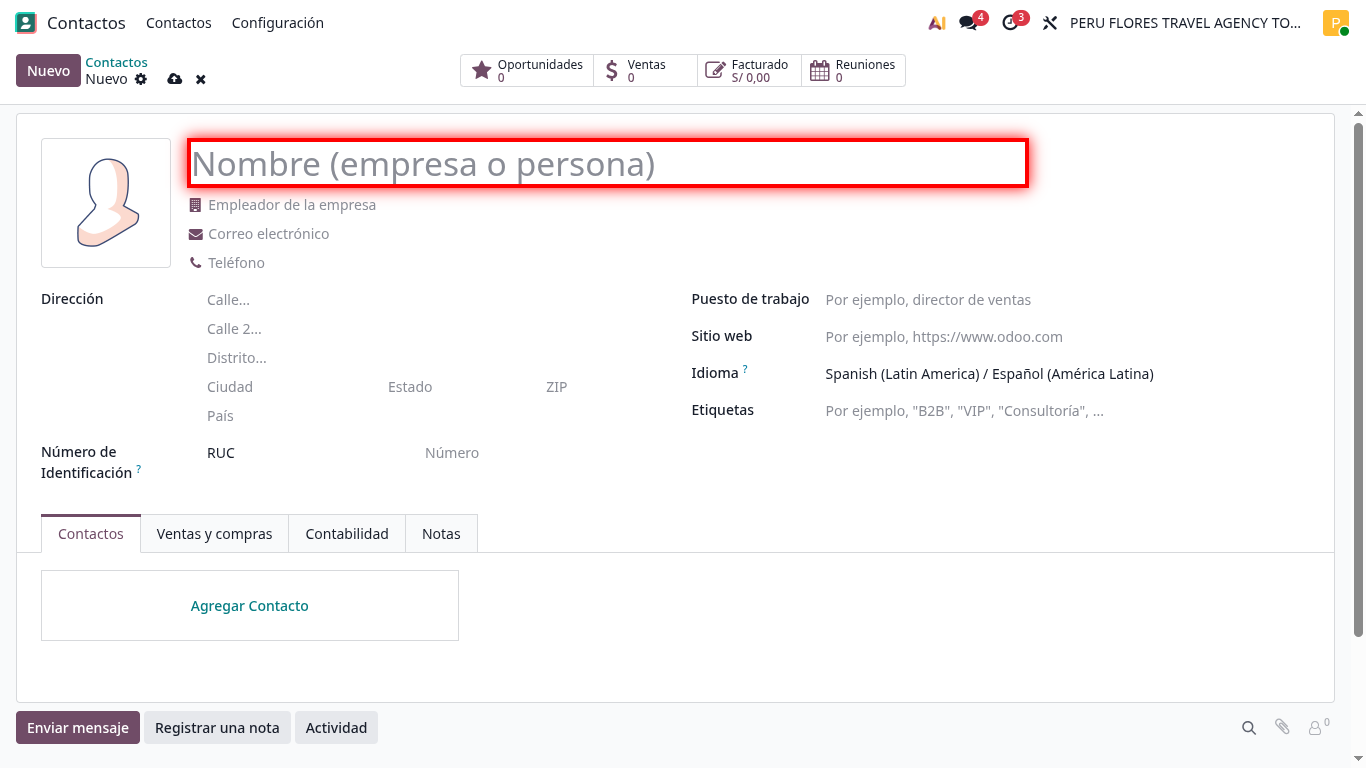
\includegraphics[width=0.9\textwidth]{assets/con_05_nombre_highlight.png}
    \caption{La ficha en blanco lista para escribir. El campo del nombre está marcado en rojo.}
\end{figure}

\begin{enumerate}
    \setcounter{enumi}{2}
    \item En el campo de arriba (marcado en rojo), escribe el \textbf{Nombre y Apellido} del cliente o el nombre de la empresa.
    \item El sistema guarda los cambios automáticamente mientras escribes, pero si ves un botón de nube en la parte de arriba, haz clic ahí para \textbf{``Guardar manualmente''}.
\end{enumerate}

% ─────────────────────────────────────────────────────────────────────────────
\subsection{Buscar y editar un contacto existente}

A veces necesitas actualizar el teléfono de alguien o simplemente encontrar su correo rápido.

\begin{figure}[H]
    \centering
    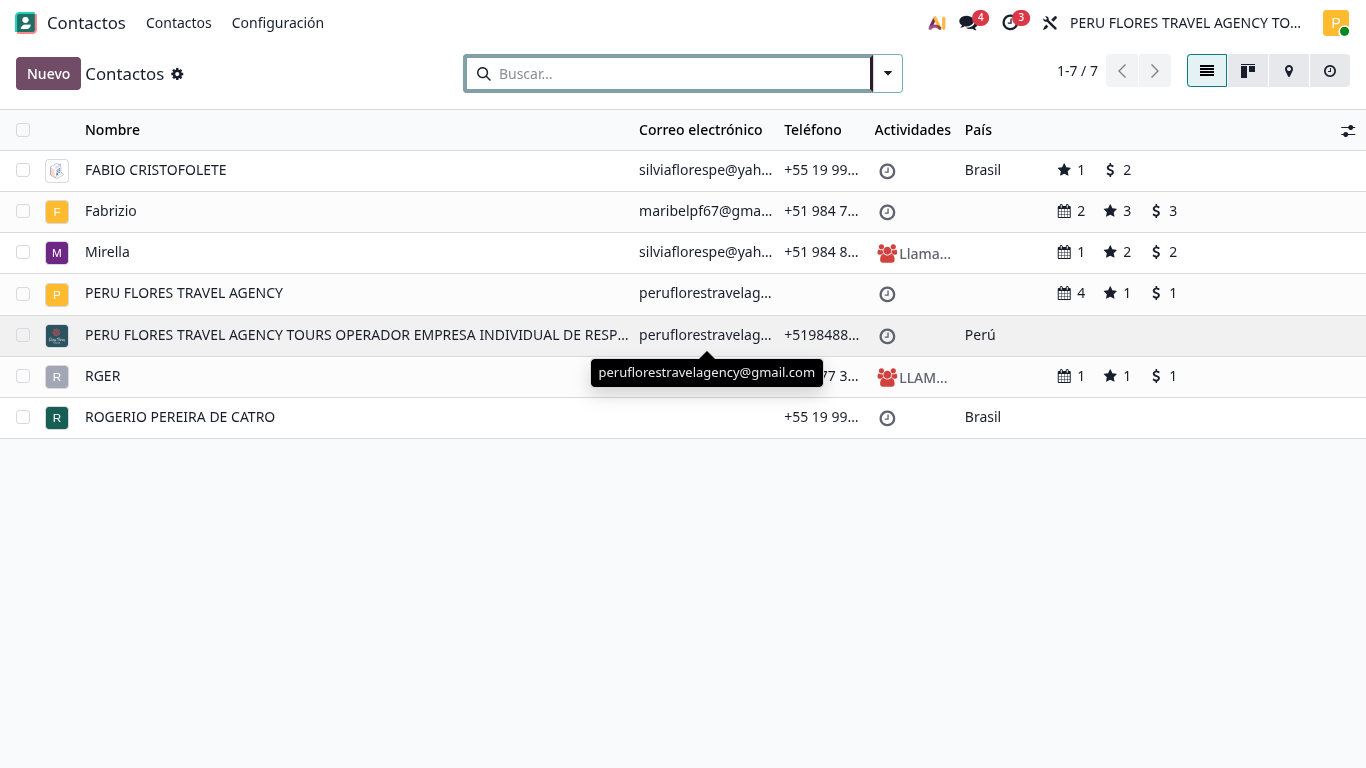
\includegraphics[width=0.9\textwidth]{assets/con_03_busqueda_highlight.png}
    \caption{La barra de búsqueda (marcada en rojo) en la parte de arriba}
\end{figure}

Sigue estos pasos:
\begin{enumerate}
    \item En la pantalla principal de Contactos, busca la barra en la parte superior derecha que tiene una lupa (marcada en rojo).
    \item Haz clic ahí y escribe el nombre de la persona que buscas.
    \item El sistema te mostrará los resultados; haz clic en el nombre que quieres abrir.
    \item Si quieres cambiar algún dato, simplemente haz clic sobre el campo (por ejemplo, el teléfono) y escribe el nuevo número.
\end{enumerate}

% ─────────────────────────────────────────────────────────────────────────────
\subsection{Ver cotizaciones, ventas y oportunidades por cliente}

Lo mejor de tener a tus clientes aquí es que el sistema te lleva la cuenta de todo lo que haces con ellos.

Sigue estos pasos:
\begin{enumerate}
    \item Abre la ficha de cualquier cliente.
    \item En la parte superior verás unos botones con íconos.
    \item Estos botones te dicen cuántas \textbf{``Oportunidades''}, \textbf{``Ventas''} o \textbf{``Facturas''} tienes con esa persona.
    \item Haz clic en cualquiera de esos botones para ver el detalle. Por ejemplo, si haces clic en ``Ventas'', verás todas las compras que te ha hecho.
\end{enumerate}

% ─────────────────────────────────────────────────────────────────────────────
\subsection{Pestañas y chatter útiles}

En la ficha del contacto, abajo de los datos principales, verás varias pestañas y una zona especial a la derecha (o abajo) llamada ``Chatter''.

\begin{itemize}
    \item \textbf{Pestaña Contactos y Direcciones:} Si el cliente es una empresa (como una Agencia), aquí puedes agregar a los vendedores o trabajadores de esa agencia.
    \item \textbf{Pestaña Ventas y Compras:} Aquí le dices al sistema si esta persona es un cliente o si es un proveedor que te vende cosas.
    \item \textbf{El Chatter (lado derecho):} Es como un historial de mensajes. Aquí puedes escribir \textbf{``Registrar una nota''} para dejar mensajes internos para tu equipo (ej. ``A este cliente le gustan los hoteles frente al mar'').
\end{itemize}

% ─────────────────────────────────────────────────────────────────────────────
\subsection{Adjuntar documentos (pasaporte u identificación)}

Es muy importante guardar copias de pasaportes o DNI de los pasajeros directamente en su ficha.

\begin{figure}[H]
    \centering
    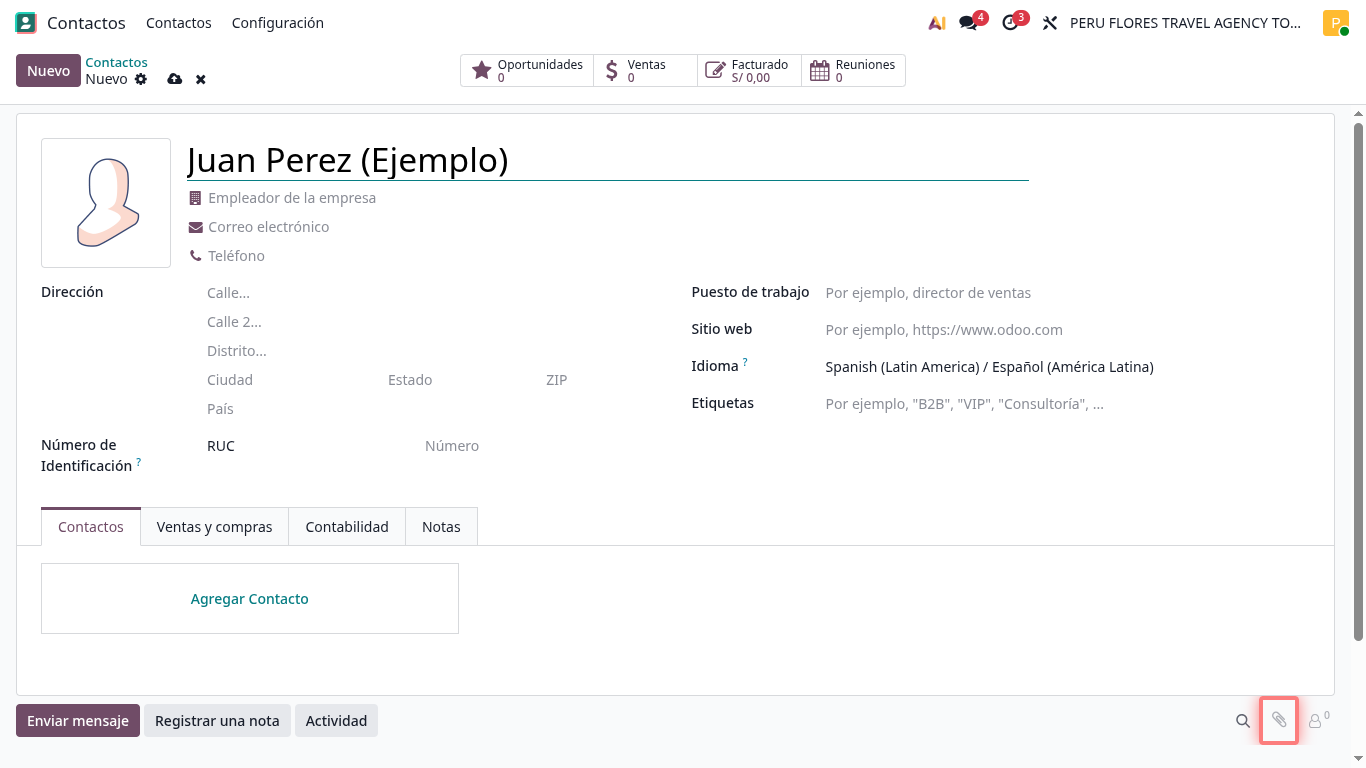
\includegraphics[width=0.9\textwidth]{assets/con_06_adjuntar_highlight.png}
    \caption{El botón con el ícono de clip (marcado en rojo) en el Chatter}
\end{figure}

Sigue estos pasos:
\begin{enumerate}
    \item En la ficha del cliente, ve al lado derecho (al Chatter).
    \item Busca el ícono que parece un \textbf{clip de papel} (marcado en rojo).
    \item Haz clic ahí, busca el PDF o la foto del pasaporte en tu computadora y súbelo.
    \item El documento quedará guardado para siempre en la ficha del pasajero.
\end{enumerate}

% ─────────────────────────────────────────────────────────────────────────────
\subsection{Datos mínimos que debe capturar para cada cliente (PAX o contacto operativo)}

Para que todo funcione bien cuando vendas un paquete turístico, acostúmbrate a pedir siempre estos datos mínimos:

\begin{itemize}
    \item \textbf{Nombre completo:} Para que los boletos de tren y entradas salgan correctos.
    \item \textbf{Correo electrónico:} Para poder enviarle cotizaciones, confirmaciones y la encuesta de satisfacción.
    \item \textbf{Teléfono o WhatsApp:} Para contactarlo rápido si hay algún cambio en el tour.
    \item \textbf{Nacionalidad / Tipo de Documento:} Clave para saber qué tarifas aplican en boletos turísticos o trenes.
\end{itemize}

% ─────────────────────────────────────────────────────────────────────────────
\subsection{Relación con el CRM (siguiente capítulo)}

Ahora que sabes cómo guardar clientes, el siguiente paso lógico es venderles algo. Cuando un cliente guardado te pide información sobre un tour, eso se convierte en una \textbf{``Oportunidad''}. En el siguiente capítulo veremos cómo usar el sistema CRM para convertir esas oportunidades en ventas cerradas y dinero.
